% THIS DOCUMENT FOLLOWS THE VOLERE TEMPLATE BY Suzanne Robertson and James Robertson
% ONLY THE SECTION HEADINGS ARE PROVIDED
%
% Initial draft from https://github.com/Dieblich/volere
%
% Risks are removed because they are covered by the Hazard Analysis
\documentclass[12pt]{article}

\usepackage{booktabs}
\usepackage{tabularx}
\usepackage{longtable}
\usepackage{hyperref}
\usepackage{graphicx}

\hypersetup{
    bookmarks=true,         % show bookmarks bar?
    colorlinks=true,        % false: boxed links; true: colored links
    linkcolor=red,          % color of internal links (change box color with linkbordercolor)
    citecolor=green,        % color of links to bibliography
    filecolor=magenta,      % color of file links
    urlcolor=cyan           % color of external links
}

\newcommand{\lips}{\textit{Insert your content here.}}

%% Comments

\usepackage{color}

\newif\ifcomments\commentstrue %displays comments
%\newif\ifcomments\commentsfalse %so that comments do not display

\ifcomments
\newcommand{\authornote}[3]{\textcolor{#1}{[#3 ---#2]}}
\newcommand{\todo}[1]{\textcolor{red}{[TODO: #1]}}
\else
\newcommand{\authornote}[3]{}
\newcommand{\todo}[1]{}
\fi

\newcommand{\wss}[1]{\authornote{blue}{SS}{#1}} 
\newcommand{\plt}[1]{\authornote{magenta}{TPLT}{#1}} %For explanation of the template
\newcommand{\an}[1]{\authornote{cyan}{Author}{#1}}

%% Common Parts

\newcommand{\progname}{ProgName} % PUT YOUR PROGRAM NAME HERE
\newcommand{\authname}{Team \#, Team Name
\\ Student 1 name
\\ Student 2 name
\\ Student 3 name
\\ Student 4 name} % AUTHOR NAMES                  

\usepackage{hyperref}
    \hypersetup{colorlinks=true, linkcolor=blue, citecolor=blue, filecolor=blue,
                urlcolor=blue, unicode=false}
    \urlstyle{same}
                                


\begin{document}

\title{Software Requirements Specification for \progname} 
\author{\authname}
\date{\today}
	
\maketitle

~\newpage

\pagenumbering{roman}

\tableofcontents

~\newpage

\section*{Revision History}

\begin{tabularx}{\textwidth}{p{3cm}p{2cm}X}
\toprule
\textbf{Date} & \textbf{Version} & \textbf{Notes} \\
\midrule
10/11/2024 & Revision 0 & Initial draft of SRS \\
04/04/2025 & Revision 1 & Added diagrams; Fixed spelling; Added references; Added Reflection; Looked over the missing context in part 7; Rationales were looked over but no citations were used (hence no citations were added); Fixed table formatting; Added additional context to unclear sections; Removed solution based requirements; Updated all requirements based off comments and feedback from rubrics \\
\bottomrule
\end{tabularx}

~\\

~\newpage
\section{Purpose of the Project}
\subsection{User Business}
The McMaster Engineering Society is looking to develop a finance and accounting system that will streamline the financial operations of 60 student groups. Due to recent struggles in managing and keeping track of reimbursement requests, many students must endure long wait times during the process. The implementation of our solution will allow the MES to provide users with adequate tracking of reimbursement requests, reduce the loss of requests, and lower wait times.

\subsection{Goals of the Project}
Currently, the MES is losing track of reimbursement requests made, resulting in long wait times and lost money. We aim to provide a solution that effectively manages and organizes the large volume of reimbursement requests sent. The effectiveness of our solution will be measured based on how well it reduces wait times and how many requests are lost. Additionally, we plan on implementing custom budget creation and tracking for all users. Through this, users will be able to effectively create and manage budgets for different categories, and all transactions will be tracked in real time. This will allow users to gain financial oversight, ultimately preventing them from going over budget. Custom budgets should be categorized correctly nine times out of ten. The system should also reduce reimbursement turnover time for users, improving the claim process. Finally, the solution should be easy for users to understand and use. There should be an intuitive way to create reimbursement requests, and if required, users will be provided with extra instructions where needed.

\section{System Overview} 
In this section, the system architecture and general flow of how users will interact with the system are detailed.  

\begin{figure}[h!]
  \centering
  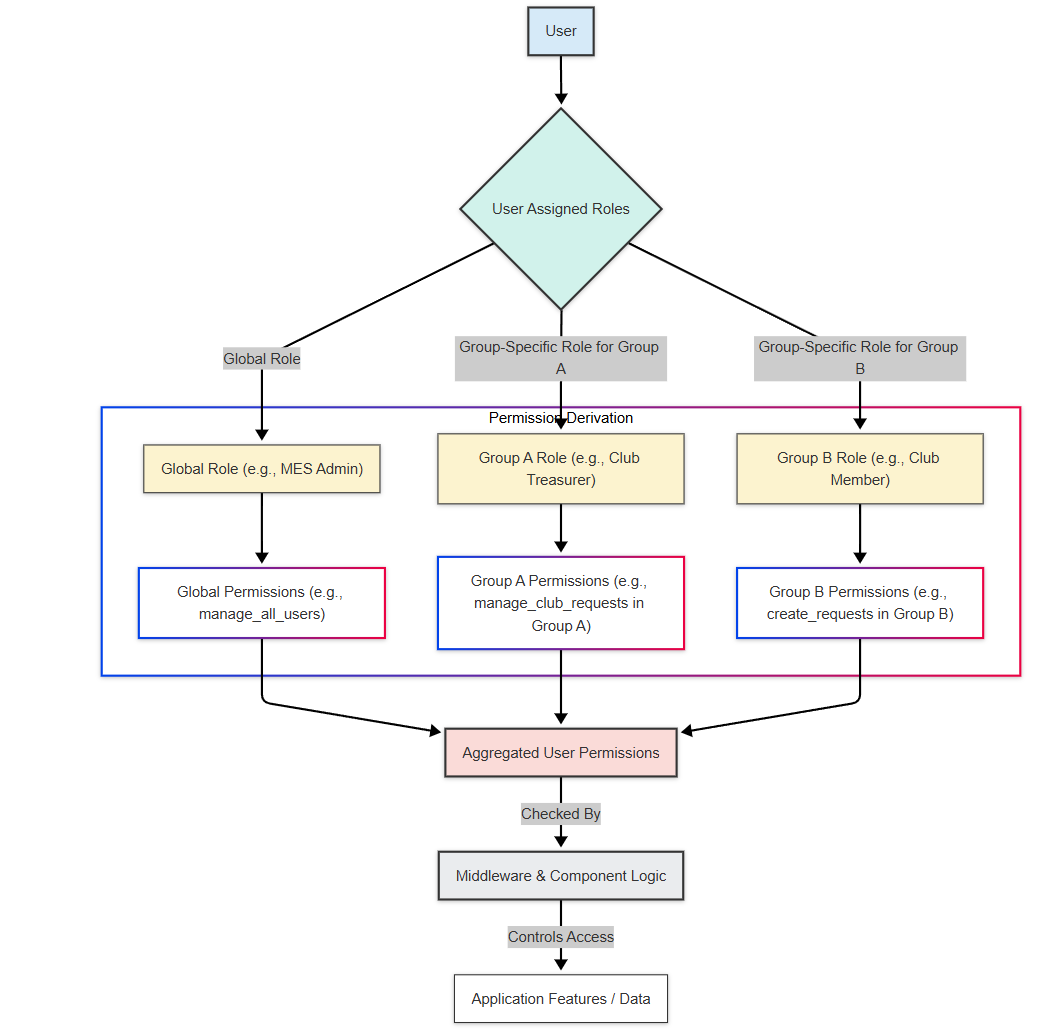
\includegraphics[width=1\textwidth]{system_detail.png}
  \caption{System process from different users}
  \label{fig:detailed-architecture}
\end{figure}

\clearpage

\begin{figure}[h!]
  \centering
  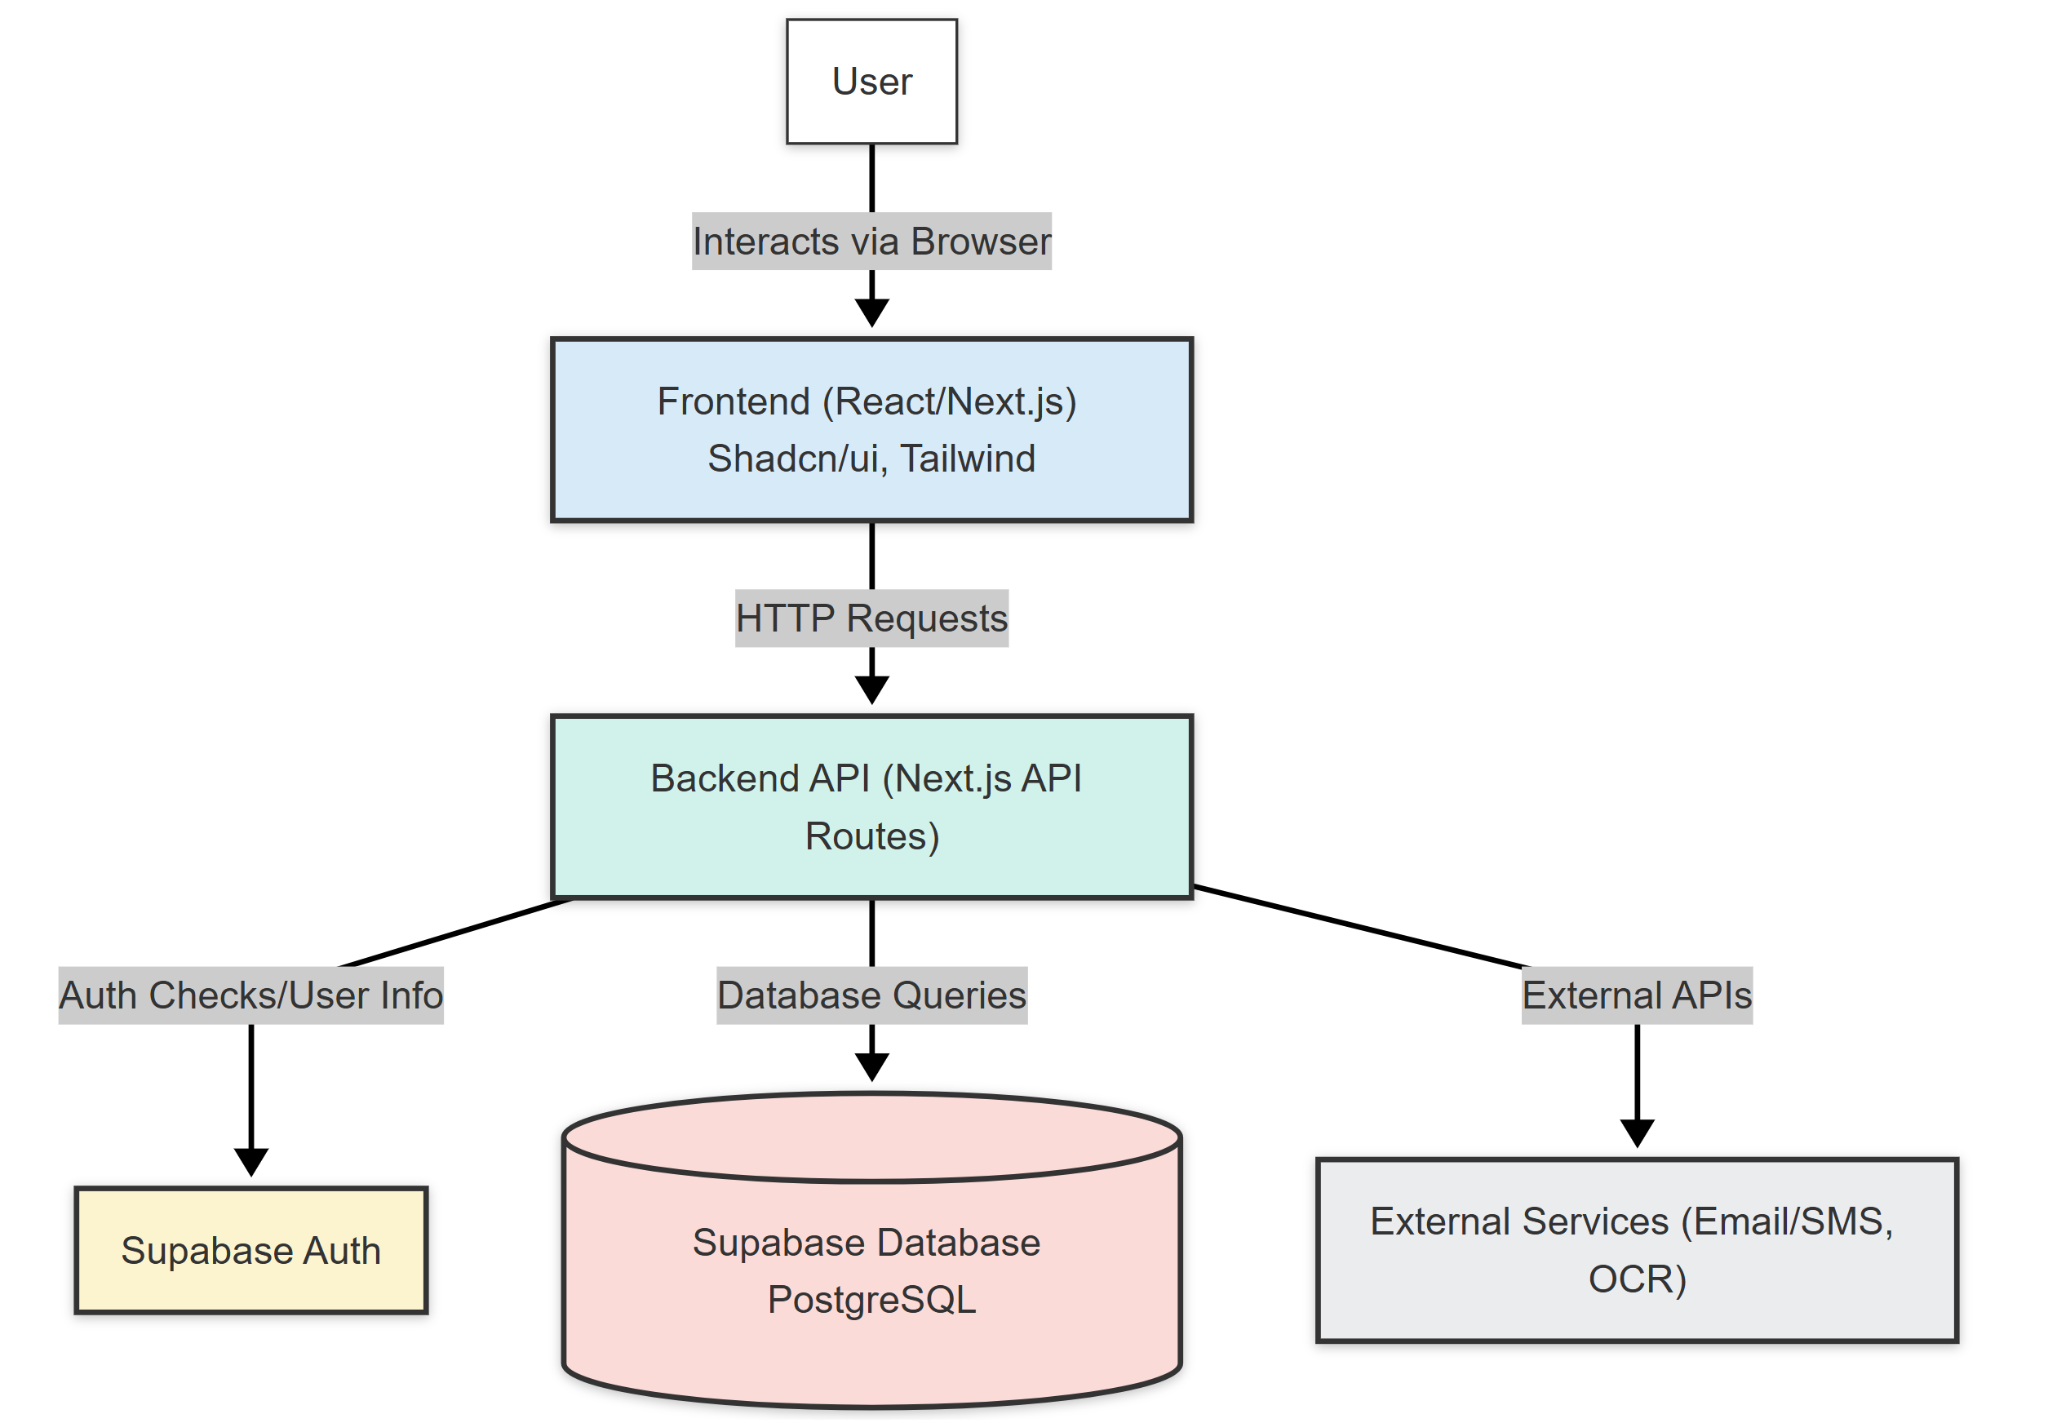
\includegraphics[width=1\textwidth]{stack.png}
  \caption{System Architecture}
  \label{fig:stack-architecture}
\end{figure}

\section{Stakeholders}
\subsection{Client}
The client for this project is the McMaster Engineering Society (MES). The MES financially supports 60 different student groups and numerous individuals throughout the year through a reimbursement model. The society is responsible for approving the final product and ensuring it meets the needs of the student groups.
The MES invests in this platform to streamline financial processes, reduce administrative overhead, and improve user experience for students and administrators.

\textbf{Roles and responsibilities:} 
\begin{itemize}
    \item Maintain the server that will host the tool
    \item Process and complete the reimbursement requests
\end{itemize}

\subsection{Customer}
The primary customers of this platform are the student groups and administrative personnel who utilize the reimbursement system. Their roles and responsibilities include:
\begin{itemize}
    \item \textbf{Expense Submission:} Student leaders and members submit expense reports via a user-friendly interface.
    \item \textbf{Feedback Providers:} Provide feedback on system usability and required features.
    \item \textbf{User Adoption:} Their willingness to adopt the system affects overall success.
\end{itemize}

\subsection{Other Stakeholders}
Other stakeholders include individuals and groups that may influence or be impacted by the product:
\begin{itemize}
    \item \textbf{Student Group Leaders:} Provide insights into the specific needs and challenges faced in the current reimbursement process.
    \item \textbf{MES Administrative Staff:} Assist in processing reimbursements and will need training on the new system to ensure smooth operations.
    \item \textbf{McMaster Administration:} May want to ensure that the tool follows relevant standards and policies.
    \item \textbf{Club Members:} Occasionally submit expense receipts and will want an easy experience.
    \item \textbf{MES IT:} Involved in integration with existing systems and maintenance.
\end{itemize}

\subsection{Hands-On Users of the Project}
\begin{itemize}
    \item \textbf{Student Leaders:} Typically aged 18-25, manage club finances, need an intuitive interface.
    \item \textbf{Administrators:} MES staff aged 18-25, require tools for efficient review/approval workflows.
    \item \textbf{Financial Administrators:} Experienced professionals (30+), need advanced financial compliance and reporting features.
\end{itemize}

\subsection{Personas}
\begin{itemize}
  \item \textbf{Alex, the Student Leader (20):} Seeks time-saving features for reimbursements.
  \item \textbf{Jamie, the MES Administrator (21):} Values accuracy and clear approval workflows.
  \item \textbf{James, the VP Finance (22):} Prefers tools providing high-level summaries and robust reports.
  \item \textbf{Jordan, the Club Member (19):} Submits occasional claims, wants straightforward UI.
\end{itemize}

\subsection{Priorities Assigned to Users}
\begin{itemize}
    \item \textbf{Key Users:} Student leaders; they must easily submit expenses.
    \item \textbf{Secondary Users:} MES administrators; essential for approvals but secondary to consistent submissions.
    \item \textbf{Unimportant Users:} Casual users; their requirements are considered last.
\end{itemize}

\subsection{User Participation}
\begin{itemize}
    \item \textbf{Requirements Gathering:} Interviews and surveys with key users to document the reimbursement process.
    \item \textbf{Usability Testing:} Hands-on sessions to validate design choices.
    \item \textbf{Regular Check-Ins:} Meetings to ensure alignment with user expectations.
\end{itemize}

\subsection{Maintenance Users and Service Technicians}
\begin{itemize}
    \item \textbf{MES IT Staff:} Responsible for system updates, troubleshooting, and maintenance documentation.
\end{itemize}

\section{Mandated Constraints}
\subsection{Solution Constraints}
\begin{enumerate}
  \item The system must manage reimbursement requests for 60 student groups efficiently.
  \item The system must track and display the status of each request to the submitting group.
  \item The system must allow uploading and storage of receipt images or files.
  \item The system must be online continuously or display a clear message when offline.
\end{enumerate}

\subsection{Implementation Environment of the Current System}
\begin{enumerate}
  \item There is no existing system in place.
  \item The new system will be hosted on an MES-provided laptop or server running Windows 10 or higher, with at least 4 GB RAM and a modern GPU (e.g., RTX 2080).
\end{enumerate}

\subsection{Partner or Collaborative Applications}
\begin{enumerate}
  \item N/A (No partner or collaborative application exists for this project).
\end{enumerate}

\subsection{Off-the-Shelf Software}
\begin{enumerate}
  \item An external API may be used for scanning receipts; the final choice is pending.
\end{enumerate}

\subsection{Anticipated Workplace Environment}
\begin{enumerate}
  \item Development will occur on local machines with Git for version control and collaboration.
\end{enumerate}

\subsection{Schedule Constraints}
\begin{enumerate}
  \item Final demonstration is set for April 2nd, serving as the primary deadline for core features.
\end{enumerate}

\subsection{Budget Constraints}
\begin{enumerate}
  \item The budget is capped at \$750 for the entire project.
\end{enumerate}

\subsection{Enterprise Constraints}
\begin{enumerate}
  \item All developed code and documentation will be owned by the MES.
\end{enumerate}

\section{Naming Conventions and Terminology}
\subsection{Glossary of All Terms, Including Acronyms, Used by Stakeholders Involved in the Project}

\begin{itemize}
    \item \textbf{MES}: McMaster Engineering Society.   
    \item \textbf{Audit Log}: A record of actions performed within the system, noting the user, action, and time.
    \item \textbf{Club Financial Manager}: A designated club member overseeing financial records and reimbursement submissions.
    \item \textbf{Budget Allocation}: The amount of funding designated for specific clubs or activities, used to track and control spending.
    \item \textbf{Vendor Contracts}: Agreements with external suppliers for goods or services.
    \item \textbf{Approval Workflow}: The process a reimbursement request undergoes from submission to final approval.
    \item \textbf{Financial Dashboard}: A system feature providing an overview of budgets, reimbursements, and pending actions.
    \item \textbf{CI/CD}: Continuous Integration/Continuous Deployment for automated testing and code deployment.
\end{itemize}

\section{Relevant Facts And Assumptions}
\subsection{Relevant Facts}
\begin{itemize}
  \item No existing application is currently handling these reimbursements.
  \item The project targets 60 student groups at McMaster University.
  \item The system design must allow for future growth and additional features.
\end{itemize}

\subsection{Business Rules}
\begin{itemize}
  \item Users receive notifications when their submitted receipts are reimbursed.
  \item Users are notified in advance of any scheduled maintenance windows.
  \item All financial records are stored on the backend for reference and auditing.
\end{itemize}

\subsection{Assumptions}
\begin{itemize}
  \item The MES provides the server hardware for hosting the system.
  \item The MES supplies any data required for testing and validation.
  \item Reliable internet connectivity is assumed for normal usage and notifications.
\end{itemize}

\section{The Scope of the Work}
\subsection{The Current Situation}
Currently, the MES manages reimbursements through manual methods such as Google Forms, PDFs, and spreadsheets, causing delays, lost requests, and difficulty tracking finances.

\subsection{The Context of the Work}
The MES-ERP project aims to streamline these financial processes by enabling a single platform for reimbursement requests, budget oversight, and comprehensive reporting. This includes an audit trail for transaction histories.

\subsection{Work Partitioning}
\begin{itemize}
  \item \textbf{Reimbursement Submission Module:} Allows users to upload receipts and request reimbursements.
  \item \textbf{Reimbursement Review and Approval:} Administrators approve or reject pending requests.
  \item \textbf{Audit and Compliance Module:} Maintains an audit log for all actions and financial records.
  \item \textbf{Budget/User Dashboards:} Provides real-time tracking of budgets, spending, and request statuses.
\end{itemize}

\subsection{Specifying a Business Use Case (BUC)}
\textbf{BUC 1: Submitting a Reimbursement Request}  
\begin{itemize}
  \item \textbf{Precondition:} User has valid credentials and receipts.
  \item \textbf{Trigger:} A club needs reimbursement for an authorized expense.
  \item \textbf{Steps:}
  \begin{enumerate}
      \item User logs into MES-ERP.
      \item User navigates to `Submit Reimbursement.'
      \item User completes required fields and uploads receipts.
      \item User submits the request.
  \end{enumerate}
  \item \textbf{Postcondition:} Request is placed in the approval queue.
\end{itemize}

\textbf{BUC 2: Reviewing a Reimbursement Request}  
\begin{itemize}
  \item \textbf{Precondition:} A request has been submitted.
  \item \textbf{Trigger:} An MES administrator checks the pending requests or receives a notification.
  \item \textbf{Steps:}
  \begin{enumerate}
      \item Administrator logs in.
      \item Administrator navigates to pending requests.
      \item Administrator reviews details and receipts.
      \item Administrator approves or rejects the request with optional feedback.
  \end{enumerate}
  \item \textbf{Postcondition:} Request status is updated for the submitter to view.
\end{itemize}

\section{Business Data Model and Data Dictionary}
\subsection{Business Data Model}
The MES-ERP system manages financial and user-related data across several entities:

\begin{itemize}
    \item \textbf{User Entity:}
    \begin{itemize}
        \item \textbf{Attributes:} UserID, Name, Email, Group, Role, Phone Number
        \item \textbf{Relationships:} A user may submit multiple reimbursement requests; roles determine permissions.
    \end{itemize}
    
    \item \textbf{Reimbursement Request Entity:}
    \begin{itemize}
        \item \textbf{Attributes:} RequestID, Timestamp, SubmitterID, Amount, Status, Attached Receipts
        \item \textbf{Relationships:} Each request is linked to a single user; administrators can review or modify the status.
    \end{itemize}
    
    \item \textbf{Budget Entity:}
    \begin{itemize}
        \item \textbf{Attributes:} BudgetID, GroupID, TotalAmountAllocated, AmountSpent, Category
        \item \textbf{Relationships:} A group manages one budget, with possible multiple spending entries or reimbursement references.
    \end{itemize}

    \item \textbf{Group Entity:}
    \begin{itemize}
        \item \textbf{Attributes:} GroupID, GroupName, CreatedAt
        \item \textbf{Relationships:} A group can have multiple associated users and budgets.
    \end{itemize}
    
    \item \textbf{Role Entity:}
    \begin{itemize}
        \item \textbf{Attributes:} RoleID, RoleName
        \item \textbf{Relationships:} Determines which system actions are allowed (e.g., submit, approve).
    \end{itemize}

\end{itemize}

\subsection{Data Dictionary}
N/A (No additional data dictionary provided at this time).

\section{The Scope of the Product}
\subsection{Product Boundary}
\begin{itemize}
    \item \textbf{Automated Functions:}
    \begin{itemize}
        \item Reimbursement request submission
        \item Notification of updates and statuses
        \item Approval/rejection workflow
        \item Basic budget tracking
    \end{itemize}
    \item \textbf{Manual Functions:}
    \begin{itemize}
        \item Legacy data entry for older records
        \item User training and support
        \item Handling of non-digital (physical) receipts
    \end{itemize}
\end{itemize}

\subsection{Product Use Case Table}
\begin{table}[h]
  \centering
  \caption{Product Use Case Summary Table}
  \resizebox{\textwidth}{!}{%
  \begin{tabular}{|c|l|l|l|}
      \hline
      \textbf{PUC No} & \textbf{PUC Name} & \textbf{Actor/s} & \textbf{Input \& Output} \\ \hline
      1 & Submit Reimbursement Request & Student Leader & (in) Reimbursement details \newline (out) Confirmation message \\ \hline
      2 & Review Reimbursement Requests & Administrator & (in) Request details \newline (out) Approved/Rejected status \\ \hline
      3 & Track Payment Requests & Administrator & (in) Payment info \newline (out) Payment status \\ \hline
      4 & Process Funding Applications & Student Leader & (in) Funding application \newline (out) Approval status \\ \hline
      5 & Save Repetitive Information & Student Leader & (in) User data \newline (out) Data saved confirmation \\ \hline
      6 & Send Notifications & System & (in) Event triggers \newline (out) Emails/SMS notifications \\ \hline
      7 & Manage Audit Trails & Financial Auditor & (in) Search/Filter criteria \newline (out) Audit trail report \\ \hline
  \end{tabular}%
  }
\end{table}

\subsection{Individual Product Use Cases (PUCs)}
\textbf{PUC 1: Submit Reimbursement Request}  
\textbf{Actors:} Student Leader  
\textbf{Scenario:} A student leader submits an expense reimbursement request with attached receipts.

\textbf{PUC 2: Review Reimbursement Requests}  
\textbf{Actors:} Administrator  
\textbf{Scenario:} An administrator reviews and decides on a submitted request.

\textbf{PUC 3: Track Payment Requests}  
\textbf{Actors:} Administrator  
\textbf{Scenario:} An administrator verifies the status of paid or pending reimbursements.

\textbf{PUC 4: Process Funding Applications}  
\textbf{Actors:} Student Leader  
\textbf{Scenario:} A student leader submits an application for intramural or special funding.

\textbf{PUC 5: Save Repetitive Information}  
\textbf{Actors:} Student Leader  
\textbf{Scenario:} A user stores frequently used data (address, contact info) to simplify future submissions.

\textbf{PUC 6: Send Notifications}  
\textbf{Actors:} System  
\textbf{Scenario:} Automated notifications when request statuses change or approvals occur.

\textbf{PUC 7: Manage Audit Trails}  
\textbf{Actors:} Financial Auditor  
\textbf{Scenario:} Auditor reviews logs to ensure compliance or investigate anomalies.

\section{Functional Requirements}
\subsection{Functional Requirements}

\begin{itemize}

  \item \textbf{Requirement Number}: 001  
  \item \textbf{Description}: The system must allow club financial managers (or authorized users) to submit reimbursement requests with attached receipts.  
  \item \textbf{Rationale}: Without a submission feature, expenses cannot be recorded, delaying financial processes and risking lost receipts.  
  \item \textbf{Fit Criterion}:  
  \begin{itemize}
    \item A user with the “Club Financial Manager” role can upload receipts and complete a reimbursement form.
    \item The new request must appear in the system’s pending queue at least 95\% of the time without errors.
  \end{itemize}
  \item \textbf{Priority}: High  
  \item \textbf{Originator}: Club Financial Manager
  
  \bigskip

  \item \textbf{Requirement Number}: 002  
  \item \textbf{Description}: The system must allow MES staff to approve or reject reimbursement requests, updating the status accordingly.  
  \item \textbf{Rationale}: Administrators require an approval workflow to finalize reimbursements; otherwise, requests cannot be processed or escalated.  
  \item \textbf{Fit Criterion}:  
  \begin{itemize}
    \item An administrator can change a request’s status to Approved or Rejected.
    \item The change must reflect in the database and be visible to the submitter.
  \end{itemize}
  \item \textbf{Priority}: High  
  \item \textbf{Originator}: MES Finance Team

  \bigskip

  \item \textbf{Requirement Number}: 003  
  \item \textbf{Description}: The system must notify the request submitter whenever there is a change in the status of the reimbursement request.  
  \item \textbf{Rationale}: Submitters must be informed of any updates to address additional requirements or confirm approvals.  
  \item \textbf{Fit Criterion}:  
  \begin{itemize}
    \item A notification is sent (email or user-chosen method) within 30 seconds of status change.
    \item 90\% of notifications should reach users successfully under normal conditions.
  \end{itemize}
  \item \textbf{Priority}: Medium  
  \item \textbf{Originator}: MES Finance Team

  \bigskip

  \item \textbf{Requirement Number}: 004  
  \item \textbf{Description}: The system must allow administrators to access all financial records, audit logs, and user actions for oversight.  
  \item \textbf{Rationale}: Full access is needed for auditing, compliance, and potential investigations.  
  \item \textbf{Fit Criterion}:  
  \begin{itemize}
    \item An administrator can retrieve data on any submitted reimbursement or user action without permission errors.
    \item The system must maintain at least one year’s worth of logs for each financial record.
  \end{itemize}
  \item \textbf{Priority}: High  
  \item \textbf{Originator}: System Administrators
  
\end{itemize}

\section{Look and Feel Requirements}
\subsection{Appearance Requirements}
\begin{enumerate}
  \item Animations must be minimal and only used to provide necessary feedback. \\
  \textbf{Rationale}: Minimizing animations reduces distractions and maintains clarity of purpose.
\end{enumerate}

\subsection{Style Requirements}
\begin{enumerate}
  \item The system must not include any imagery or language that is discriminatory, vulgar, or otherwise inappropriate. \\
  \textbf{Rationale}: Ensures a professional and inclusive environment.
  \item The platform should avoid high-contrast color combinations that may strain the eyes. \\
  \textbf{Rationale}: Preserves readability and user comfort.
  \item Overall tone shall be professional and formal. \\
  \textbf{Rationale}: Reinforces confidence in a financial system handling sensitive data.
  \item Form fields shall be clearly labeled, with errors highlighted in red. \\
  \textbf{Rationale}: Clear labels and error indicators reduce user confusion.
  \item Icons for navigation or key actions shall be intuitive and consistent. \\
  \textbf{Rationale}: Simplifies learning curve and speeds up task completion.
\end{enumerate}

\section{Usability and Humanity Requirements}
\subsection{Ease of Use Requirements}
\begin{enumerate}
  \item The system’s UI elements (buttons, forms, menus) shall maintain consistent styling and positioning to promote ease of learning. \\
  \textbf{Rationale}: Consistency helps new users quickly understand navigation and reduces errors.
  \item The main menu shall allow navigation to primary features in three clicks or fewer. \\
  \textbf{Rationale}: Quick navigation improves efficiency and user satisfaction.
\end{enumerate}

\subsection{Personalization and Internationalization Requirements}
\begin{enumerate}
  \item N/A (English only; no additional personalization or localization required at this stage).
\end{enumerate}

\subsection{Learning Requirements}
\begin{enumerate}
  \item The system shall provide a brief on-screen tutorial or help option for new users on their first reimbursement submission. \\
  \textbf{Rationale}: Reduces user confusion and the likelihood of errors during early usage.
\end{enumerate}

\subsection{Understandability and Politeness Requirements}
\begin{enumerate}
  \item All error messages shall include a description of the issue and a suggestion for fixing it. \\
  \textbf{Rationale}: Clear guidance on errors saves user time and reduces frustration.
\end{enumerate}

\subsection{Accessibility Requirements}
\begin{enumerate}
  \item The product shall offer a high-contrast mode for visually impaired users. \\
  \textbf{Rationale}: Ensures the platform is accessible to those with visual impairments or color blindness.
\end{enumerate}

\section{Performance Requirements}
\subsection{Speed and Latency Requirements}
\begin{itemize}
    \item The system shall respond to user actions (page loads, form submissions) within 2 seconds for 90\% of requests under normal load.
    \item Repetitive information entry or retrieval shall not exceed 1 second in typical usage scenarios.
\end{itemize}

\subsection{Safety-Critical Requirements}
\begin{itemize}
  \item N/A (No immediate life-critical functionality; focus is on data security and accuracy).
\end{itemize}

\subsection{Precision or Accuracy Requirements}
\begin{itemize}
    \item All monetary values must be stored and displayed with two decimal places.
    \item The system shall validate numerical fields to prevent data entry errors (e.g., non-numeric amounts).
\end{itemize}

\subsection{Robustness or Fault-Tolerance Requirements}
\begin{itemize}
    \item The system shall back up financial records daily to prevent loss from system failures or corruption.
\end{itemize}

\subsection{Capacity Requirements}
\begin{itemize}
    \item The system shall support at least 200 concurrent users during peak usage without a noticeable slowdown.
    \item The database must store up to five years of financial transactions without performance degradation.
\end{itemize}

\subsection{Scalability or Extensibility Requirements}
\begin{itemize}
    \item The system shall allow for adding new user roles or additional student groups without a major redesign of the database schema.
\end{itemize}

\subsection{Longevity Requirements}
\begin{itemize}
    \item The product shall be maintainable for at least five years under a defined maintenance budget.
\end{itemize}

\section{Operational and Environmental Requirements}
\subsection{Expected Physical Environment}
\begin{enumerate}
  \item The system will be used primarily in indoor office settings, with stable power and networking. 
\end{enumerate}

\subsection{Wider Environment Requirements}
\begin{enumerate}
  \item The system is intended to replace manual methods (Google Forms, spreadsheets) for MES reimbursements.
\end{enumerate}

\subsection{Requirements for Interfacing with Adjacent Systems}
\begin{enumerate}
  \item The system must be accessible from Windows, Mac, and Linux devices, supporting at least the last four versions of major browsers (Chrome, Firefox, Edge).
\end{enumerate}

\subsection{Productization Requirements}
\begin{enumerate}
  \item N/A (The product is not for external sale).
\end{enumerate}

\subsection{Release Requirements}
\begin{enumerate}
  \item The product shall be tested for regressions before each official release. 
  \item Critical bugs must be addressed and resolved before a new version is deployed to production.
\end{enumerate}

\section{Maintainability and Support Requirements}
\subsection{Maintenance Requirements}
\begin{enumerate}
  \item The system must allow for future reimbursement process changes or an increase in student groups without needing a complete redesign. \\
  \textbf{Rationale}: Ensures the software remains adaptable as MES operations evolve.
  \item The codebase and technical documentation must enable a new developer to address general maintenance issues within one week of onboarding. \\
  \textbf{Rationale}: Proper documentation and clear structure shorten learning curves for support staff.
\end{enumerate}

\subsection{Supportability Requirements}
\begin{enumerate}
  \item The system must run on MES-authorized devices meeting a minimum of Windows 10, 4 GB RAM, and stable internet connectivity. \\
  \textbf{Rationale}: Standard hardware and networking reduce support complexity.
\end{enumerate}

\subsection{Adaptability Requirements}
\begin{enumerate}
  \item The system must handle scaling from 60 clubs to at least 100 clubs if the MES expands. \\
  \textbf{Rationale}: Accommodates future growth without major refactoring.
\end{enumerate}

\section{Security Requirements}
\subsection{Access Requirements}
\begin{enumerate}
  \item Administrators must have full privileges to view, modify, or delete all financial records, user roles, and audit logs. \\
  \textbf{Rationale}: Necessary for oversight, auditing, and compliance checks.
  \item Club financial managers shall only access or modify data relevant to their own club. \\
  \textbf{Rationale}: Protects privacy and data integrity across different clubs.
\end{enumerate}

\subsection{Integrity Requirements}
\begin{enumerate}
  \item All modifications to financial records must be logged with user ID, timestamp, and action details. \\
  \textbf{Rationale}: Ensures traceability of changes for audit and compliance.
\end{enumerate}

\subsection{Privacy Requirements}
\begin{enumerate}
  \item The system must adhere to PIPEDA, ensuring personal data is handled securely and only for authorized purposes. \\
  \textbf{Rationale}: Protects user data and aligns with legal standards.
  \item Users should be able to request corrections or removal of their personal data if allowed by MES policies. \\
  \textbf{Rationale}: Respects user rights and privacy.
\end{enumerate}

\subsection{Audit Requirements}
\begin{enumerate}
  \item The system must generate exportable logs detailing each significant financial action, from request submission to final approval. \\
  \textbf{Rationale}: Facilitates investigations and historical record-keeping for compliance.
\end{enumerate}

\subsection{Immunity Requirements}
\begin{enumerate}
  \item All third-party libraries must be reviewed monthly for updates or security patches. \\
  \textbf{Rationale}: Minimizes exposure to known vulnerabilities.
\end{enumerate}

\section{Cultural Requirements}
\subsection{Cultural Requirements}
\begin{enumerate}
  \item The interface language shall be English, using British spelling if conflict arises. \\
  \textbf{Rationale}: Aligns with McMaster University’s regional norms.
  \item Inclusive language shall be used to avoid cultural bias or assumptions about users. \\
  \textbf{Rationale}: Reflects the diversity of MES’s student population.
\end{enumerate}

\section{Compliance Requirements}
\subsection{Legal Requirements}
\begin{itemize}
    \item \textbf{Data Protection Compliance:} Must comply with PIPEDA for data collection, storage, and consent.
    \item \textbf{Accessibility Compliance:} Follow AODA guidelines for an inclusive user experience.
\end{itemize}

\subsection{Standards Compliance Requirements}
\begin{itemize}
    \item \textbf{Information Security Standards:} Align with ISO/IEC 27001 best practices for managing sensitive information.
    \item \textbf{Software Development Standards:} Adhere to Agile principles for iterative development and stakeholder feedback.
\end{itemize}

\section{Open Issues}
\begin{itemize}
  \item \textbf{Issue Number}: 001  
  \item \textbf{Cross-reference}: FR-003 (Notifications)  
  \item \textbf{Summary}: Determining whether to send notifications via email, SMS, or in-app alerts.  
  \item \textbf{Stakeholders Involved}: Project Team, MES IT Team  
  \item \textbf{Action}: Conduct a survey or meeting to finalize the preferred method.  
  \item \textbf{Resolution}: Expected within one week.

  \bigskip

  \item \textbf{Issue Number}: 002  
  \item \textbf{Cross-reference}: FR-004 (Audit Logs)  
  \item \textbf{Summary}: Retention period for audit logs is unclear.  
  \item \textbf{Stakeholders Involved}: Project Team, MES IT Team  
  \item \textbf{Action}: Decide data retention policy in alignment with MES financial guidelines.  
  \item \textbf{Resolution}: Expected within two weeks.

  \bigskip

  \item \textbf{Issue Number}: 003  
  \item \textbf{Cross-reference}: FR-002 (Approval Workflow)  
  \item \textbf{Summary}: Thresholds for multi-level approvals (e.g., high-value requests) are undefined.  
  \item \textbf{Stakeholders Involved}: Project Team, MES Finance Team  
  \item \textbf{Action}: Define rules and thresholds for multi-level approvals.  
  \item \textbf{Resolution}: Expected within two weeks.

  \bigskip
\end{itemize}

\section{Off-the-Shelf Solutions}
\subsection{Ready-Made Products}
\begin{enumerate}
  \item N/A (No existing product meets MES-specific needs).
\end{enumerate}

\subsection{Reusable Components}
\begin{enumerate}
  \item Existing UI libraries and receipt parsing APIs can be integrated.
\end{enumerate}

\subsection{Products That Can Be Copied}
\begin{enumerate}
  \item Some budgeting app UIs can inspire design but will require custom adaptation to MES workflows.
\end{enumerate}

\section{New Problems}
\subsection{Effects on the Current Environment}
\begin{itemize}
    \item Training might be needed as users transition away from manual systems.
    \item Historical data remains in spreadsheets unless explicitly imported.
\end{itemize}

\subsection{Effects on the Installed Systems}
\begin{itemize}
    \item Must ensure hardware/software compatibility with existing MES infrastructure.
    \item Temporary hybrid usage (old and new) may occur during transition.
\end{itemize}

\subsection{Potential User Problems}
\begin{itemize}
    \item Resistance to change from familiar manual processes.
    \item Errors if new users find the interface confusing.
\end{itemize}

\subsection{Limitations in the Anticipated Implementation Environment That May Inhibit the New Product}
\begin{itemize}
    \item Server capacity may become an issue at peak load, requiring upgrades.
    \item Network outages or limited bandwidth could hinder usage.
\end{itemize}

\subsection{Follow-Up Problems}
\begin{itemize}
    \item Need for additional training if advanced features or expansions are introduced.
    \item Possible legal/policy changes affecting how finances are tracked.
\end{itemize}

\section{Tasks}
\subsection{Project Planning}
An Agile approach (e.g., Scrum) will be used to iteratively refine requirements and deliverables.

\subsection{Planning of the Development Phases}
\begin{longtable}{| m{3cm} | m{10cm} |}
  \hline
  \textbf{Step} & \textbf{Description} \\
  \hline
  \textbf{1. Requirements Gathering} & Ongoing collaboration with stakeholders to define user stories and acceptance criteria. \\
  \hline
  \textbf{2. Sprint Planning} & Select and prioritize tasks from the backlog for each 1--4 week sprint. \\
  \hline
  \textbf{3. Design and Architecture} & Establish initial data models and system design, refining as needed. \\
  \hline
  \textbf{4. Development} & Implement features, coordinating with testers for immediate feedback. \\
  \hline
  \textbf{5. Testing} & Conduct unit, integration, and user acceptance tests within each sprint. \\
  \hline
  \textbf{6. Review and Retrospective} & Evaluate completed work, gather stakeholder feedback, and identify improvements for the next sprint. \\
  \hline
  \textbf{7. Release Planning} & Decide on feature packages and when to deploy them to production. \\
  \hline
  \textbf{8. Continuous Feedback} & Stakeholder input guides future sprints, ensuring alignment with evolving needs. \\
  \hline
\end{longtable}

\subsection{Requirement Priority}

The following outlines the priority levels for each category of requirements in this SRS, along with brief rationales. These priorities guide the order in which features should be addressed during development when resources (time, budget) are constrained.

\begin{itemize}

    \item \textbf{Functional Requirements (Highest Priority)} \\
    \textbf{Rationale:} Core functionalities like request submission, approval workflows, and admin oversight (FR-001, FR-002, FR-003, and FR-004) form the backbone of the system. Without these features, the MES cannot handle reimbursements effectively.

    \item \textbf{Security and Privacy Requirements (High Priority)} \\
    \textbf{Rationale:} Financial data is sensitive. Ensuring controlled access, encryption, and adherence to legal standards (e.g., PIPEDA) is critical to user trust and regulatory compliance. Security failures can severely undermine the system’s viability.

    \item \textbf{Compliance Requirements (High Priority)} \\
    \textbf{Rationale:} Meeting legal (PIPEDA, AODA) and industry standards (ISO/IEC 27001) is non-negotiable for a financial platform. Non-compliance can lead to legal repercussions and reputational damage.

    \item \textbf{Performance Requirements (Medium–High Priority)} \\
    \textbf{Rationale:} The system must reliably manage peak loads and handle concurrent users. While performance optimization can occur iteratively, unacceptable lag or downtime would undermine user confidence and adoption.

    \item \textbf{Usability and Accessibility Requirements (Medium Priority)} \\
    \textbf{Rationale:} A user-friendly interface and features like high-contrast mode encourage adoption and reduce errors. Though essential for overall success, these can be refined after the core reimbursement logic is in place.

    \item \textbf{Look and Feel Requirements (Medium Priority)} \\
    \textbf{Rationale:} Maintaining a clean, professional interface supports a positive user experience, especially important for financial transactions. However, basic functionality and security must still take precedence.

    \item \textbf{Maintainability and Support Requirements (Medium Priority)} \\
    \textbf{Rationale:} Ensuring the codebase is well-documented and easily extensible will save time and costs in the long run, especially if MES processes change or the platform expands to serve more groups. While it may not block initial launch, neglecting maintainability increases technical debt.

    \item \textbf{Operational and Environmental Requirements (Medium Priority)} \\
    \textbf{Rationale:} The system’s environment (offices, MES-provided hardware) and adjacency to other processes (e.g., budget committees, cloud backups) must be stable to avoid downtime. This stability underpins successful day-to-day usage.

    \item \textbf{Cultural Requirements (Low–Medium Priority)} \\
    \textbf{Rationale:} Respectful, inclusive language and British spelling (as required by McMaster conventions) are important but do not hinder core financial workflows. These can be verified or adjusted without blocking core features.

    \item \textbf{Longevity Requirements (Medium Priority)} \\
    \textbf{Rationale:} Building the system to last at least five years is valuable for ROI and operational continuity; however, it can be balanced with immediate functional needs and iterative improvements.

\end{itemize}

\section{Migration to the New Product}
\subsection{Requirements for Migration to the New Product}
N/A --- No official migration of legacy data is currently mandated. Historical files remain in their existing formats unless otherwise requested.

\subsection{Data That Has to be Modified or Translated for the New System}
N/A --- No translation of old data is required for the first release. Further data integration can be explored later.

\section{Costs}
\subsection{Labor Costs}
\begin{itemize}
    \item \textbf{Development Hours}: Estimated 400--500 hours to implement key features (reimbursement flow, approvals, budgeting).
    \item \textbf{Testing Hours}: Estimated 50--70 hours for comprehensive testing (unit, integration, acceptance).
\end{itemize}

\subsection{Monetary Costs}
\begin{itemize}
    \item \textbf{Server Operating Costs}: \$10--\$20 monthly for electricity and basic upkeep of MES’s local server.
\end{itemize}

\subsection{Additional Considerations}
\begin{itemize}
    \item \textbf{Maintenance Costs}: 5--10 hours monthly for bug fixes and feature updates.
    \item \textbf{Backup Budget}: 10--20 hours set aside for unforeseen issues or requirement changes.
\end{itemize}

\section{Likely Changes}
Potential future additions include:
\begin{enumerate}
  \item A mobile app for instant expense submission.
  \item Machine learning-based receipt categorization to minimize manual data entry.
  \item Customizable dashboards for different user roles.
  \item Multi-language support to serve a broader community.
  \item Historical data import from prior systems.
\end{enumerate}

\section{Ideas for Solution}
A web-based finance and accounting solution using JavaScript, NextJS, React, and Git is proposed to handle the MES’s reimbursement challenges:
\begin{itemize}
    \item Streamlines submission with digital receipts and real-time status tracking.
    \item Offers automated notifications for both submitters and administrators.
    \item Includes budget oversight and multiple approval levels to prevent lost requests.
\end{itemize}
TypeScript will serve as the main language. NextJS handles front-end and back-end, with React providing a responsive, interactive UI. Git supports version control for collaborative development.

\newpage{}
\section*{References}

\begin{flushleft}
Hunter, C. (n.d.). \textit{Software Requirements Specification (SRS)} [PDF]. GitHub.
\url{https://github.com/cer-hunter/OAR-CAS741/blob/main/docs/SRS/SRS.pdf}

\vspace{1em}

McMaster Engineering Society. (n.d.). \textit{Home}.
\url{https://macengsociety.ca/}
\end{flushleft}

\newpage{}
\section*{Appendix --- Reflection}

The information in this section will be used to evaluate the team members on the
graduate attribute of Lifelong Learning. Please answer the following questions:

\begin{enumerate}
  \item \textbf{What knowledge and skills will the team collectively need to acquire to
  successfully complete this capstone project?}

  As a team, we must acquire technical and domain-specific knowledge, as well as relevant soft skills. Key areas include:
  \begin{itemize}
    \item \textbf{Domain-Specific Knowledge:} Understanding the MES’s financial workflows, budgeting cycles, and typical expense categories.
    \item \textbf{Frontend Development:} Building intuitive and responsive user interfaces with React.
    \item \textbf{Backend and Database Management:} Managing data securely and in real time, possibly using NextJS and Supabase.
    \item \textbf{Project Management:} Using Agile processes and Git for efficient collaboration and consistent code quality.
  \end{itemize}

  \item \textbf{For each of the knowledge areas and skills identified in the previous
  question, what are at least two approaches to acquiring the knowledge or mastering the skill? Which will the team pursue, and why?}

  \begin{itemize}
    \item \textbf{Domain-Specific Knowledge}
    \begin{itemize}
      \item Interview MES finance staff and student leaders to understand current workflows.
      \item Examine existing reimbursement documents and spreadsheets.
      \item \textit{Chosen Approach:} Direct interviews to obtain real-world context and pain points.
    \end{itemize}

    \item \textbf{Frontend Development}
    \begin{itemize}
      \item Complete online tutorials or short courses in React.
      \item Build a small prototype and gather feedback from typical users.
      \item \textit{Chosen Approach:} Prototype-based learning to identify usability issues early.
    \end{itemize}

    \item \textbf{Backend and Database Management}
    \begin{itemize}
      \item Study official Supabase and PostgreSQL documentation.
      \item Implement a proof-of-concept backend to test data flow and security.
      \item \textit{Chosen Approach:} Hands-on experimentation to confirm performance and reliability before scaling.
    \end{itemize}

    \item \textbf{Project Management}
    \begin{itemize}
      \item Use GitHub Projects, Kanban boards, or Scrum boards for sprint planning.
      \item Conduct frequent reviews and retrospectives with stakeholders.
      \item \textit{Chosen Approach:} An Agile framework enabling iterative feedback, ensuring the final product meets evolving needs.
    \end{itemize}
  \end{itemize}
\end{enumerate}

\end{document}
